\documentclass{standalone}
\usepackage{pgfplots}
\usepackage{lmodern}
\pgfplotsset{compat=1.17}

\begin{document}
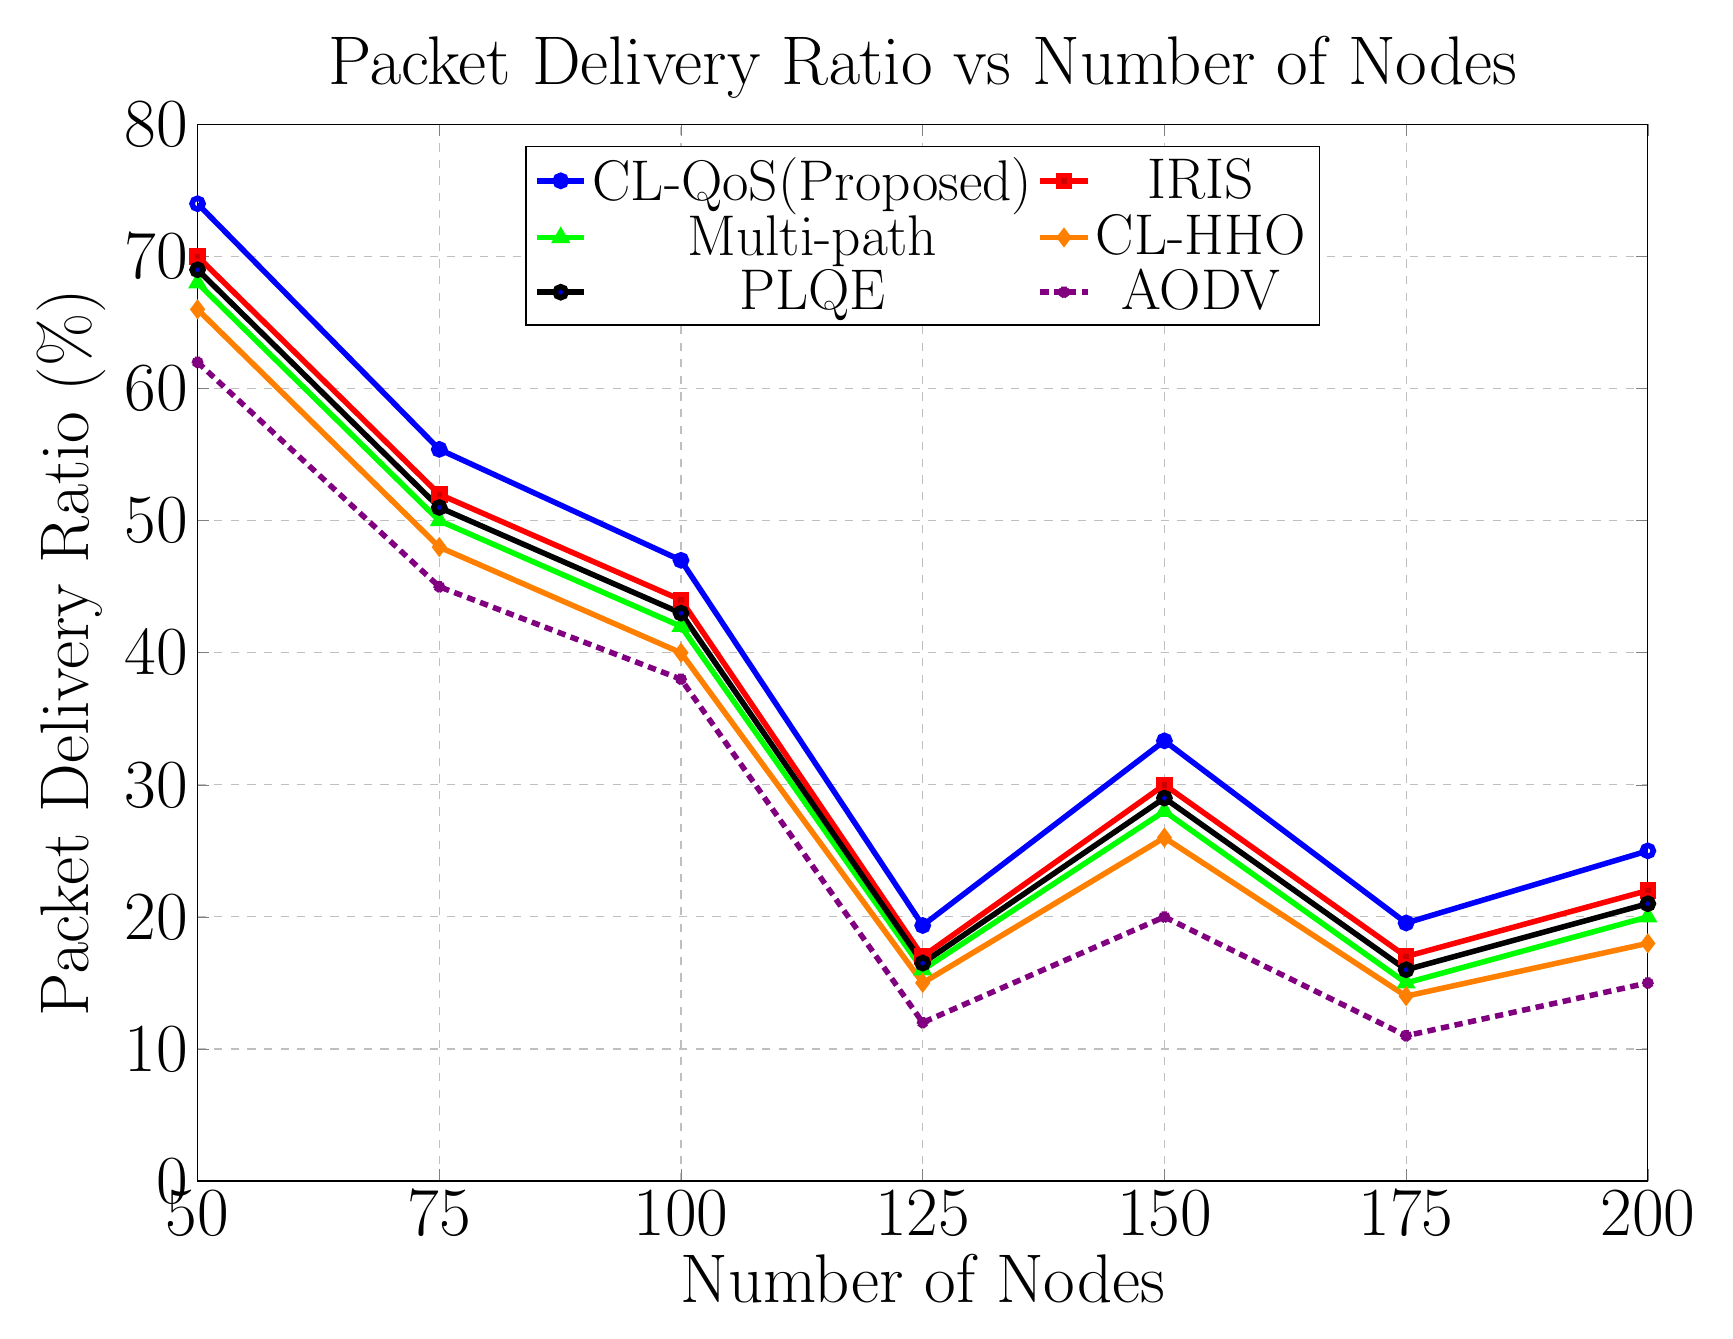
\begin{tikzpicture}
\begin{axis}[
    width=20cm,
    height=15cm,
    tick label style={font=\fontsize{24}{28}\selectfont},
    label style={font=\fontsize{24}{28}\selectfont},
    title style={font=\fontsize{24}{28}\selectfont},
    title={Packet Delivery Ratio vs Number of Nodes},
    xlabel={Number of Nodes},
    ylabel={Packet Delivery Ratio (\%)},
    xmin=50, xmax=200,
    ymin=0, ymax=80,
    xtick={50,75,100,125,150,175,200},
    ytick={0,10,20,30,40,50,60,70,80},
    legend columns=2,
    legend style={
    font=\fontsize{22}{26}\selectfont,
    at={(0.5,0.98)},
    anchor=north,
    draw=black,
    fill=white
    },
    ymajorgrids=true,
    xmajorgrids=true,
    grid style=dashed
]

% CL-QoS (REAL DATA)
\addplot+[mark=o,color=blue,line width=2pt] coordinates {
    (50,74)(75,55.4)(100,47)(125,19.35)(150,33.33)(175,19.54)(200,25)
};

% IRIS (slightly lower)
\addplot+[mark=square*,color=red,line width=2pt] coordinates {
    (50,70)(75,52)(100,44)(125,17)(150,30)(175,17)(200,22)
};

% Multi-path
\addplot+[mark=triangle*,color=green,line width=2pt] coordinates {
    (50,68)(75,50)(100,42)(125,16)(150,28)(175,15)(200,20)
};

% CL-HHO
\addplot+[mark=diamond*,color=orange,line width=2pt] coordinates {
    (50,66)(75,48)(100,40)(125,15)(150,26)(175,14)(200,18)
};

% PLQE
\addplot+[mark=*,color=black,line width=2pt] coordinates {
    (50,69)(75,51)(100,43)(125,16.5)(150,29)(175,16)(200,21)
};

% AODV
\addplot+[mark=star,color=violet,line width=2pt] coordinates {
    (50,62)(75,45)(100,38)(125,12)(150,20)(175,11)(200,15)
};

\legend{CL-QoS(Proposed), IRIS, Multi-path, CL-HHO, PLQE, AODV}

\end{axis}
\end{tikzpicture}
\end{document}